%!TEX option = -shell-escape
%!TEX builder = latexmk
%!TEX program = xelatex
\documentclass{beamer}
% ----- Loadings -----
\newif\ifcompile\compilefalse
\usetheme[menuwidth={0.7\paperwidth}]{erlangen}
\setbeamercovered{transparent=8}
\graphicspath{{./figures/}}
\usepackage{xeCJK}
\usepackage{hologo}
\usepackage{multicol}
\usepackage{tipa}
\usepackage{hyperref}
\usepackage{amsmath}
\usepackage{amssymb}
\usepackage{filecontents}
\usepackage{minted}

% ----- Font Set -----
\setCJKmainfont[AutoFakeSlant, BoldFont = FZHTK.TTF]{FZZDXK.TTF}
\setCJKmonofont[AutoFakeSlant, AutoFakeBold]{FZFSK.TTF}
% ----- New Commands -----
\newcommand{\ChinaTeX}{China\hologo{TeX}}
\renewcommand{\TeX}{\hologo{TeX}}
\renewcommand{\LaTeX}{\hologo{LaTeX}}
\renewcommand{\eTeX}{\hologo{eTeX}}
\newcommand{\pdfTeX}{\hologo{pdfTeX}}
\newcommand{\XeTeX}{\hologo{XeTeX}}
\newcommand{\LuaTeX}{\hologo{LuaTeX}}
\newcommand{\ConTeXt}{\hologo{ConTeXt}}
\newcommand{\BibTeX}{\hologo{BibTeX}}
\newcommand{\MiKTeX}{\hologo{MiKTeX}}
\newcommand{\TeXLive}{\TeX{} Live}
\newcommand{\pTeX}{p\TeX}
\newcommand{\upTeX}{up\TeX}
\newcommand{\eupTeX}{\ensuremath{\varepsilon}-up\TeX}
\newcommand{\OMEGA}{Omega}
\newcommand{\pTeXng}{\pTeX{}-ng}
\newcommand{\CTeX}{\ensuremath{\mathbb{C}}\TeX}
\newcommand{\MacTeX}{Mac\TeX}
\newcommand{\LaorTeX}{(\hologo{La})\TeX}
\makeatletter
\newcommand{\mheader}[1]{\gdef\@cm@header{#1}}
\makeatother
\newcommand{\pkg}[1]{\textsf{#1}}
\setbeamertemplate{background}{}
\setlength{\parskip}{0.5ex}
\usemintedstyle{perldoc}

% ----- Title Set -----
\title[第一篇文章]{\ChinaTeX{} 在线培训课程}
\subtitle{第一篇文章}
\author{Liam Huang}
\date{\today}
\institute{Shandong University\\[-0.2em]{\small School of Mathematics}}
\mheader{\ChinaTeX{} 在线培训课程}

\begin{filecontents*}{ex01.tex}
% 载入文档类型,`article' 表示
% 我们要写一篇「文章」。
\documentclass{article}
% 输入「标题」等信息
\title{What a Wonderful World}
\author{Liam Huang}
\date{\today}
% 标识文章开始
\begin{document}
% 输出标题
\maketitle
% 正文内容
Hello, the wonderful world!

Happy \TeX ing!

中文不会出现在 PDF 文档中。
% 标识文章结束
\end{document}
\end{filecontents*}
\begin{filecontents*}{ex01-compile.tex}
\documentclass{article}
\usepackage{geometry}
\geometry{a6paper}
\title{What a Wonderful World}
\author{Liam Huang}
\date{\today}
\begin{document}
\maketitle
Hello, the wonderful world!

Happy \TeX ing!

中文不会出现在 PDF 文档中。
\end{document}
\end{filecontents*}

\begin{filecontents*}{ex02.tex}
% 载入文档类型,`ctexart' 表示
% 我们要写一篇「中文文章」。
\documentclass[UTF8]{ctexart}
\usepackage{geometry}
\geometry{a6paper, margin = 1in}
\title{What a Wonderful World}
\author{Liam Huang}
\date{\today}
\begin{document}
\maketitle
\section{文字}
你好,美丽的世界!中文出现
在 PDF 文档中啦!
\section{数学}
\begin{equation}
  E = mc^{2}\label{eqn:mass-energy}
\end{equation}

公式 \ref{eqn:mass-energy} 是
著名的「爱因斯坦质能方程」。
\end{document}
\end{filecontents*}
\begin{filecontents*}{ex02-compile.tex}
\documentclass[UTF8]{ctexart}
\usepackage{geometry}
\geometry{a6paper, margin = 1.7cm}
\title{What a Wonderful World}
\author{Liam Huang}
\date{\today}
\begin{document}
\maketitle
\section{文字}
你好,美丽的世界!中文出现在 PDF 文档中啦!
\section{数学}
\begin{equation}
  E = mc^{2}\label{eqn:mass-energy}
\end{equation}

公式 \ref{eqn:mass-energy} 是
著名的「爱因斯坦质能方程」。
\end{document}
\end{filecontents*}

\begin{document}

\begin{frame}[plain]
  \titlepage
\end{frame}

\begin{frame}{目录}
\tableofcontents
\end{frame}

\section{\TeX{} 发展简史}

\begin{frame}
  \sectionframe{\TeX{} 发展简史}
\end{frame}

\subsection{\TeX{} 和他爹}

\begin{frame}{执拗的老爷爷}
\begin{columns}
  \begin{column}{0.45\paperwidth}
    \begin{itemize}
      \item Donald Ervin Knuth \pause
      \item 大部分 KN 的 K 不发音
        \begin{itemize}
          \item Knap (敲碎)读作 [\textipa{n\ae p}]
          \item Know (知道)读作 [\textipa{n@\textupsilon}]
        \end{itemize}
      \item Knuth 读作 [\textipa{k"nu:\texttheta}]\pause
      \item 高德纳
        \begin{itemize}
          \item 储枫(04 -- 11 年,香港城市大学计算机科学系主任)
          \item 姚期智(图灵奖;清华大学理论计算机科学研究中心主任、交叉信息研究院院长)\pause
        \end{itemize}
    \end{itemize}
  \end{column}
  \begin{column}{0.45\paperwidth}
    \begin{itemize}
      \item 1962 年开始写 The Art of Computer Programming \pause
      \item 1974 年图灵奖
      \begin{itemize}
        \item 算法分析
        \item 程序设计语言的设计
        \item 程序设计
      \end{itemize}\pause
      \item 1976 年,校对第二卷第二版时,决定开发 \TeX{}
      \item 1989 年,\TeX{} 3 成为沿用至今的稳定版本
    \end{itemize}
  \end{column}
\end{columns}
\end{frame}

\begin{frame}{执拗的老爷爷}
  \centering
  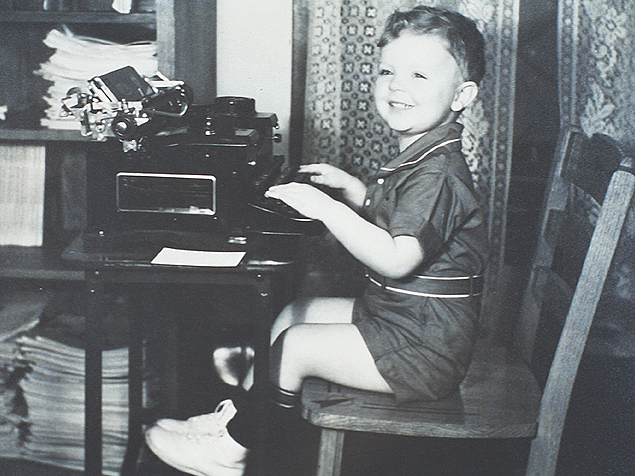
\includegraphics[width = 0.8\linewidth]{DonaldErvinKnuth_01.jpg}
\end{frame}

\begin{frame}{执拗的老爷爷}
  \centering
  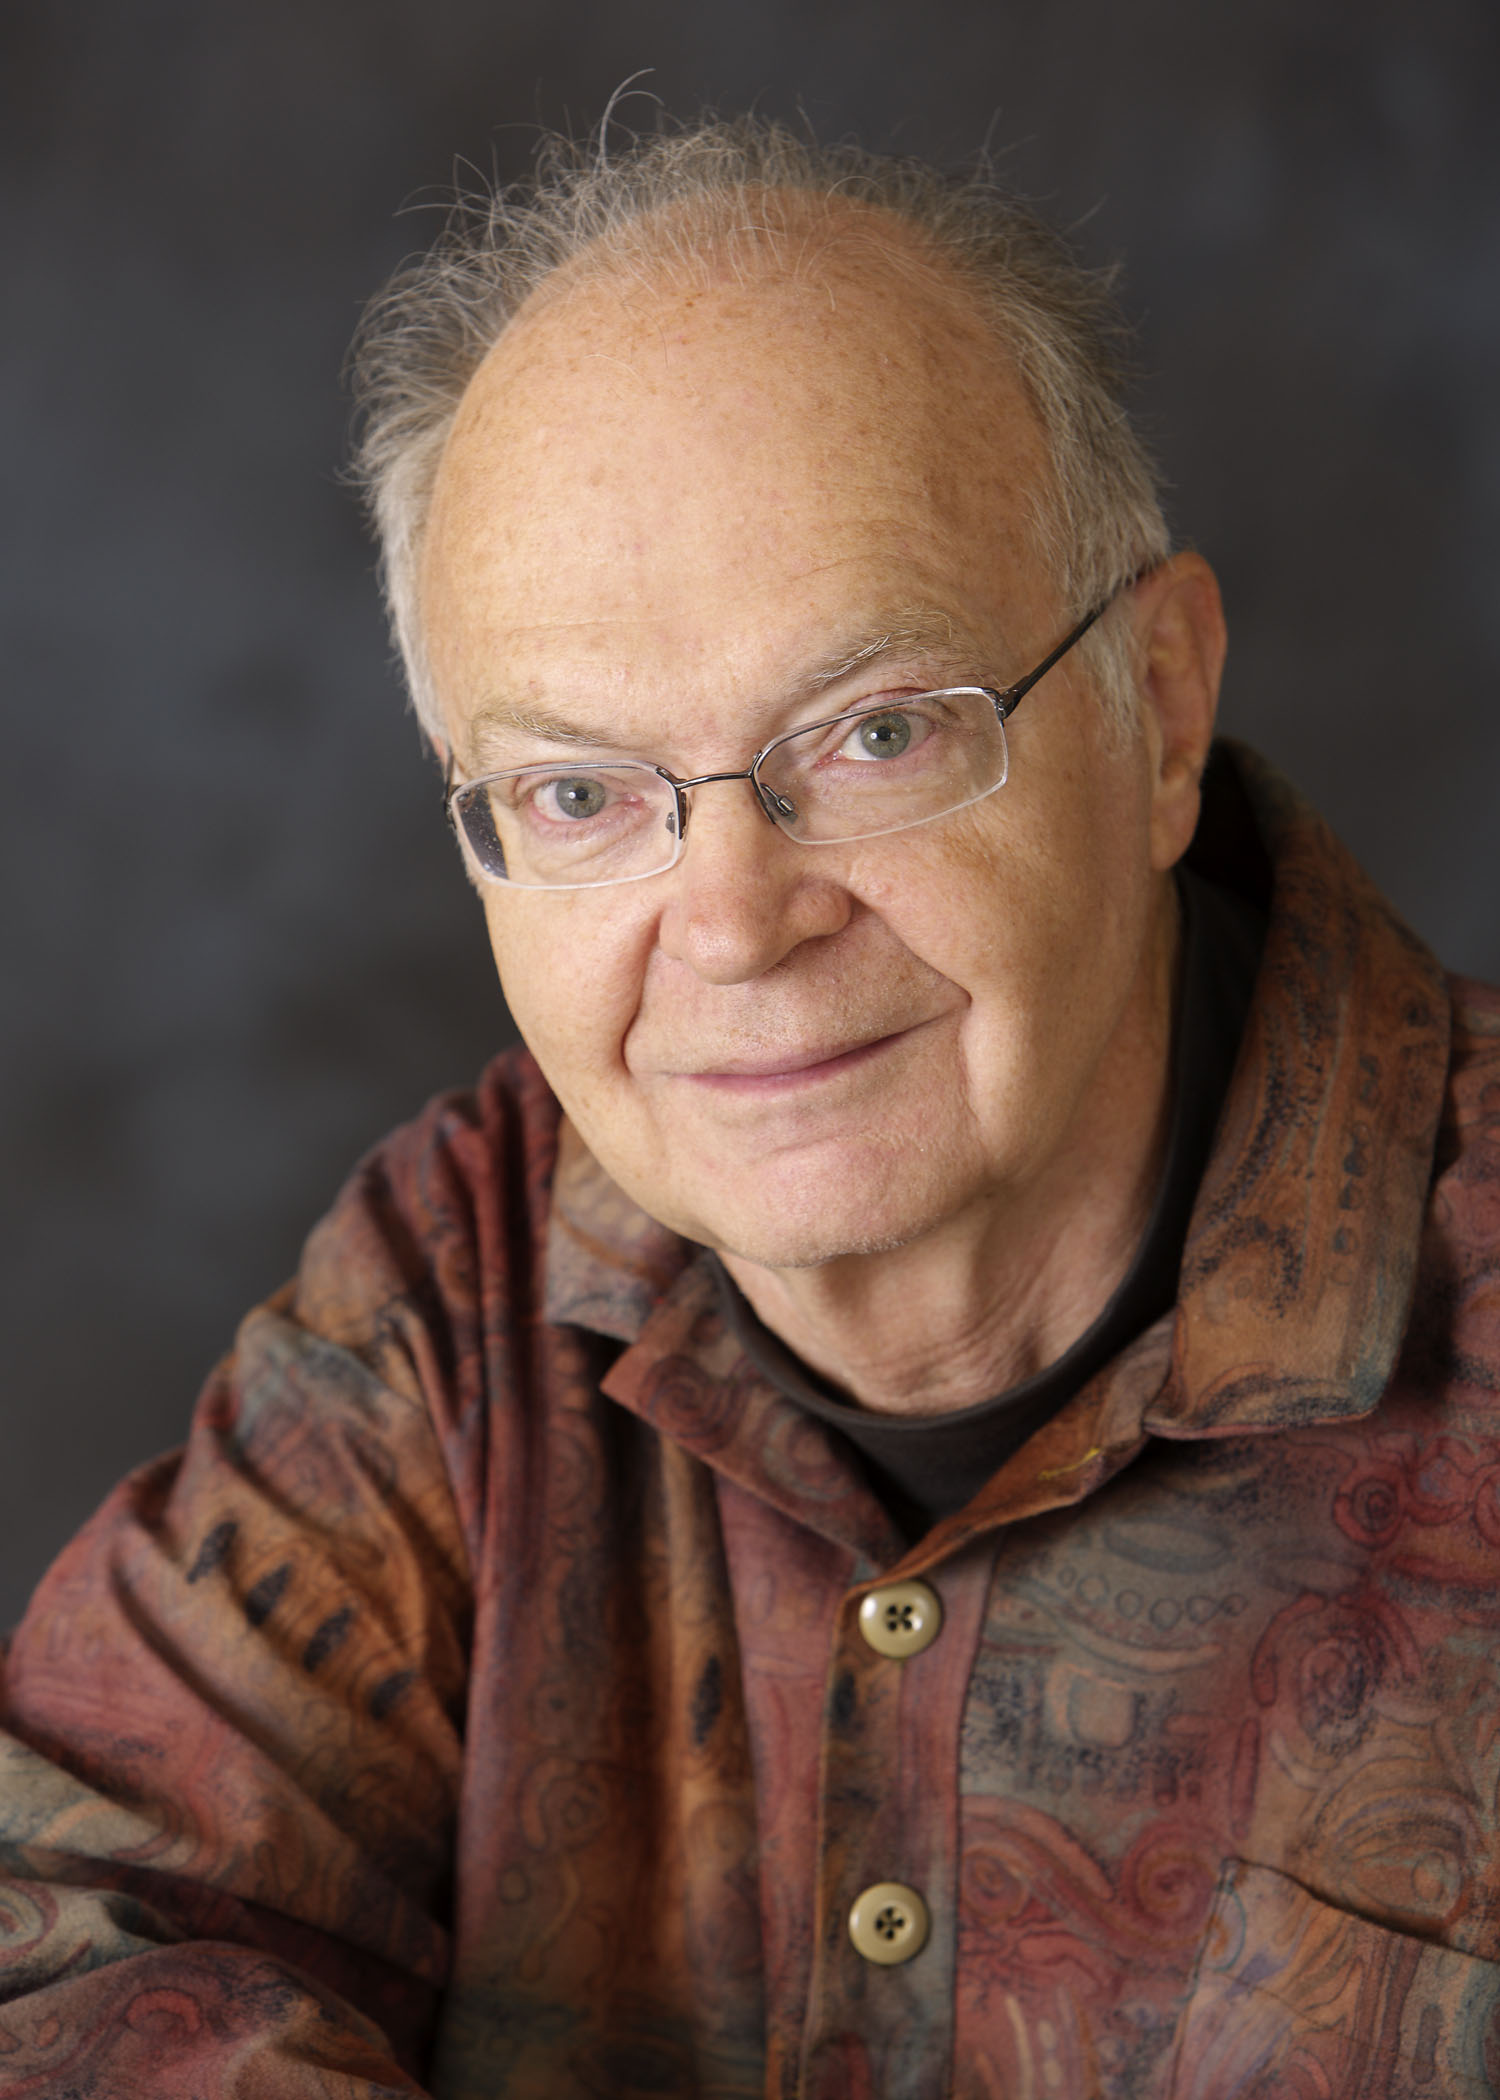
\includegraphics[height = .8\textheight]{DonaldErvinKnuth_02.jpg}
\end{frame}

\begin{frame}{此名有诗意}
  \begin{itemize}
    \item \TeX{} 是希腊词根 $\tau\epsilon\chi$ 的大写,读作 [\textipa{tEx}]
    \begin{itemize}
      \item 科技,technology
      \item 艺术
    \end{itemize}\pause
    \item E 是错位的 \pause
    \item ASCII 环境写作 TeX
  \end{itemize}
\end{frame}

\begin{frame}{\TeX{} 原语和 plain \TeX{} 格式}
  \begin{itemize}
    \item 300 多个 \TeX{} 原语(Primitives)
    \begin{itemize}
      \item 可以完成所有排版任务
      \item 晦涩难懂
    \end{itemize}\pause
    \item 600 多个宏(Macros)
    \begin{itemize}
      \item 人类可以识别的语言
    \end{itemize}
  \end{itemize}
\end{frame}

\subsection{\LaTeX{} 和他爹}

\begin{frame}{Leslie Lamport}
  \begin{columns}
    \begin{column}
      {0.45\paperwidth}
      \begin{itemize}
        \item 1941 年生于纽约
        \item 1960 年 MIT 数学学士
        \item 1963 年 Brandeis University 数学硕士,1972 年博士
      \end{itemize}
    \end{column}
    \begin{column}{0.45\paperwidth}
      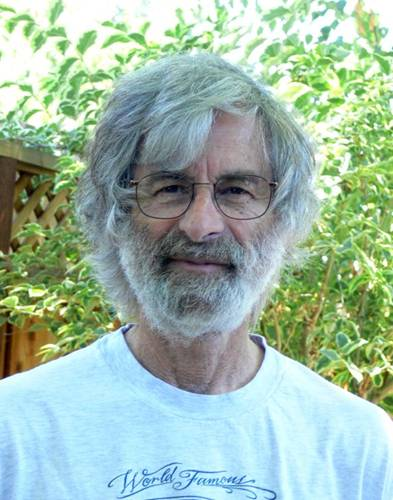
\includegraphics[height = 0.8\textheight]{Leslie_Lamport.jpg}
    \end{column}
  \end{columns}
\end{frame}

\begin{frame}{光宗耀祖}
  \begin{itemize}
    \item 1980 年代初,开发出 \LaTeX{} 格式\pause
    \begin{itemize}
      \item Lamport \TeX{}
      \item 莱氏 \TeX{}
    \end{itemize}\pause
    \item 1992 年发布 \LaTeX{} 2.09 之后撒手\pause
    \item 2001 年「叛变」到 M\$\pause
    \item 2013 年图灵奖(分散式及并形系统的理论与实践)
    \begin{itemize}
      \item 因果逻辑时序
      \item 安全性与存活度
      \item 复制状态机
      \item 循序一致性
    \end{itemize}
  \end{itemize}
\end{frame}

\section{常见发行版介绍}

\begin{frame}
  \sectionframe{常见发行版介绍}
\end{frame}

\subsection{\TeX{} 家族}

\begin{frame}
  {\TeX{} 家族}
  \begin{multicols}
    {2}
    \begin{itemize}
      \item 引擎——原语\pause
      \begin{itemize}
        \item (Knuth) TeX\pause
        \item \eTeX\pause
        \item \pdfTeX\pause
        \item \XeTeX
        \item \LuaTeX\pause
        \item \OMEGA
        \item \pTeX
        \item \upTeX, \eupTeX
        \item \pTeXng
      \end{itemize}\pause
      \item 格式——代码风格
      \begin{itemize}
        \item plain \TeX
        \item \LaTeX
        \begin{itemize}
          \item \LaTeXe
          \item \LaTeX3
        \end{itemize}
        \item \ConTeXt
      \end{itemize}\pause
      \item 宏包——某一功能\pause
      \begin{itemize}
        \item \pkg{graphicx}\pause
        \item \pkg{tabu}\pause
        \item \pkg{hyperref}\pause
        \item \pkg{fancyhdr}\pause
        \item \pkg{titlesec}\pause
        \item \pkg{natbib}
      \end{itemize}\pause
      \item 辅助工具
      \begin{itemize}
        \item \BibTeX
        \item makeindex
        \item 编辑器
      \end{itemize}\pause
      \item 发行版(套装)——上述所有内容的合集
      \begin{itemize}
        \item \MiKTeX
        \item \TeXLive
      \end{itemize}
    \end{itemize}
  \end{multicols}
\end{frame}

\begin{frame}{比喻}
  如果我们用汽车和 \TeX{} 家族来类比,那么……
  \begin{block}
    {\TeX{} 引擎是\textbf{汽车发动机}}
    \TeX{} 引擎是实际执行排版的可执行程序;正如汽车的动力归根究底来自于它的发动机。
  \end{block}
  \begin{block}
    {格式是\textbf{汽车的操纵系统}}
    格式决定了人们书写代码的方式;正如汽车的操纵系统(方向盘、离合器踏板、刹车踏板、
    油门踏板和变速箱操纵杆)决定了人们驾驶汽车的方式。
  \end{block}
\end{frame}

\begin{frame}
  {比喻}
  \begin{block}
    {宏包是\textbf{汽车的附件}}
    每个宏包都对应着一个特定的功能,没有某个宏包也能排版,但可能就有些不方便;正如
    汽车的附件(雨刷、后视镜、天窗和车载音响等),离开这些附件汽车也能行使,但总有些
    不方便。
  \end{block}
  \begin{block}
    {\TeX{} 发行版是\textbf{整辆汽车}}
    发行版中什么都有,包含运行 \TeX{} 所需的一切工具;正如一辆汽车,买来就能上路。
    不同的发行版就好像是不同品牌的汽车。
  \end{block}
\end{frame}

\subsection{\MiKTeX{} 系列}

\begin{frame}{\MiKTeX{} 系列}
  \begin{itemize}
    \item 官网:\url{http://miktex.org/}
    \item 特点
    \begin{itemize}
      \item 只支持 M\$ Windows 作业系统
      \item 有 32-bit 和 64-bit 版本
      \item 安装包小,提供即时宏包安装功能
      \item 开发者少,更新慢
    \end{itemize}\pause
    \item \CTeX
    \begin{itemize}
      \item 官网:\url{http://www.ctex.org/HomePage}
      \item 特点
      \begin{itemize}
        \item 基于 \MiKTeX{}
        \item 分为基本版和完整版
        \item 为天元系统、CCT 系统和 CJK 系统配置了字体
        \item 封装了 WinEdt 作为编辑器
      \end{itemize}
    \end{itemize}
  \end{itemize}
\end{frame}

\subsection{\TeXLive{} 系列}

\begin{frame}
  {\TeXLive{} 系列}
\begin{itemize}
  \item 官网:\url{https://www.tug.org/texlive/}
  \item 特点
  \begin{itemize}
    \item 由 TUG 维护
    \item 全平台支持
    \item 安装方式多样
    \item 开发者多,bug 少
  \end{itemize}\pause
  \item \MacTeX
  \begin{itemize}
    \item 官网:\url{https://www.tug.org/mactex/}
    \item \TeXLive{} 专为 Mac OS X 系统设计的版本
  \end{itemize}\pause
  \item 安装说明:\url{http://tieba.baidu.com/p/3524644809}
\end{itemize}
\end{frame}

\begin{frame}{FAQ}
  \begin{block}{安装完 \TeXLive{} 之后,为什么桌面上没有出现图标?}
    我们平常使用的软件安装完之后,通常会在桌面上生成一些图标,用来启动软件。
    但 \TeXLive{} 不同,它的实质是一套工具的集合。如果在桌面上生成图标,恐怕就会有
    上百甚至上千个图标。这显然是不合适的。

    用户在安装好 \TeXLive{} 之后,需要做的是使用编辑器编辑代码,然后调用
    \TeXLive{} 里的工具来编译。
  \end{block}
\end{frame}

\begin{frame}
  {FAQ}
  \begin{block}
    {我应该使用什么编辑器?}
    比较适合编辑 \LaorTeX{} 的编辑器有如下一些,你可以选择你喜欢的。
    \begin{itemize}
      \item \TeX works
      \begin{itemize}
        \item \MiKTeX 和 \TeXLive 的默认编辑器,功能简单,适合新手
      \end{itemize}
      \item \TeX shop
      \begin{itemize}
        \item \MacTeX 的默认编辑器,功能简单,适合新手
      \end{itemize}\pause
      \item \TeX maker 和 \TeX studio\pause
      \item \TeX nicCenter\pause
      \item WinEdt\pause
      \begin{itemize}
        \item 不推荐使用 \CTeX 套装里自带的 WinEdt
        \item 如果喜欢 WinEdt,可以到官网下载
      \end{itemize}\pause
      \item Vim、Emacs 和 Sublime Text
    \end{itemize}
  \end{block}
\end{frame}

\section{从简单的例子说起}

\begin{frame}
  \sectionframe{从简单的例子说起}
\end{frame}

\subsection{第一篇文档}

\begin{frame}{Hello world!}
\begin{columns}
  \begin{column}{0.45\linewidth}
    \inputminted[fontsize=\scriptsize,linenos]{tex}{ex01.tex}
  \end{column}
  \begin{column}{0.45\linewidth}
    \ifcompile\write18{xelatex ex01-compile.tex}\fi
    \fbox{\includegraphics[width = 0.96\linewidth]{ex01-compile.pdf}}
  \end{column}
\end{columns}
\end{frame}

\subsection{中文文档、数学公式、章节标题以及引用}

\begin{frame}{你好,世界!}
\begin{columns}
  \begin{column}{0.45\linewidth}
    \inputminted[fontsize=\scriptsize,linenos]{tex}{ex02.tex}
  \end{column}
  \begin{column}{0.45\linewidth}
    \ifcompile\write18{xelatex ex02-compile.tex}\fi
    \fbox{\includegraphics[width = 0.96\linewidth]{ex02-compile.pdf}}
  \end{column}
\end{columns}
\end{frame}

\section{关于提问}

\begin{frame}
  \sectionframe{关于提问}
\end{frame}

\begin{frame}{入门资料}
  绝对的新手,在提问之前请务必完整阅读一份入门资料。推荐的资料有:
  \begin{itemize}
    \item 电子文档
    \begin{itemize}
      \item \url{http://zip.ptex.tk},这是我维护的一份 \LaTeX{} 入门资料集
    \end{itemize}
    \item 商业书籍
    \begin{itemize}
      \item 《\LaTeX 入门》,刘海洋著
      \item 《\LaTeXe 完全学习手册》,胡伟著
    \end{itemize}
  \end{itemize}
\end{frame}

\begin{frame}{提问的智慧}
  \LaTeX{} 社区是热情而友好的,但请遵守社区的提问规范,基本的要求是\textbf{清晰}。
  在提问前请参考:
  \begin{itemize}
    \item \url{http://ptex.tk},这是我撰写的提问指南
  \end{itemize}
  你可以在这些地方提问:
  \begin{itemize}
    \item \CTeX 社区:\url{http://bbs.ctex.org/}
    \item \TeX{} StackExchange:\url{http://tex.stackexchange.com/}
    \item QQ 群:91940767、31752345
  \end{itemize}
\end{frame}

\section*{关于我}

\begin{frame}{关于我}
  黄晨成,毕业于山东大学数学学院,与人合著有《GRE 基础填空 24 套精析与精练》(原稿使用 \LaTeX 排版);2010 年接触 \LaTeX,是 \pkg{xprintlen} 和 \pkg{sduthesis} 宏包的作者,2013 年加入 \pkg{ctex-kit},同年与邓东升一同建立 ElegantLaTeX,发布 \pkg{ElegantBook} 等模板。

  主页:\url{http://liam0205.me}

  电邮:\href{mailto:liamhuang0205@gmail.com}{liamhuang0205@gmail.com}
\end{frame}

\end{document}
